\section{Experimental evaluation}
We evaluate the performance of the runtime decentralized enforcer synthesis framework in the context of collision-avoidance for multi-agent systems. Specifically, we use the collision-avoidance safety function defined in Scenario~3 and the pathfinder construction described in Scenario~7. 
 The implementation of the system for ensuring safety from collisions uses the general pseudocode presented in Algorithm \ref{Trajectory_update}.
 
 

\subsubsection*{Comparison with centralized shields}

We compare the modified trajectories of two agents equipped with decentralized enforcers that are synthesized at runtime with two other agents whose behaviors are modified by a centralized shield synthesized at design-time using the algorithm from Section~\ref{sec:quantshielding} in a 5x5 grid world. This algorithm runs in time that is exponential in the number  $|\mathcal{U}|$ of agents as discussed in Section~\ref{sec:quantshielding}. In general, the optimization of the plans of cooperative robots is PSPACE-hard \cite{hardness}.
The intended trajectories of the agents in both scenarios are the same. 

\begin{figure*}[!htb]
\centering
\definecolor{green1}{rgb}{0,0.6,0}
\subfloat[$t=0$]{
\begin{tikzpicture}[line join=round,x=1cm,y=1cm]
\begin{axis}[
scale=0.5,
x=1cm,y=1cm,
axis lines=middle,
ymajorgrids=true,
xmajorgrids=true,
xmin=0,
xmax=5,
ymin=0,
ymax=5,
xtick={-3,-2,...,35},
ytick={-7,-6,...,17},]

\draw [->,line width=0.6pt,color=green1] (2.2,4) -- (2.2,3);
\draw [->,line width=0.6pt,color=red,dashed] (1.8,4) -- (1.8,3);

\draw [->,line width=0.6pt,color=blue] (4,2.2) -- (3,2.2);
\draw [->,line width=0.6pt,dashed,color=red] (4,1.8) -- (3,1.8);

\begin{scriptsize}

\draw [fill=green1] (2,4) circle (1.3pt);
\draw[color=green1] (1.3,4.3) node {t=0};

\draw [fill=blue] (4,2) \Square{1.3pt};
\draw[color=blue] (4,2.5) node {t=0};

\end{scriptsize}
\end{axis}
\end{tikzpicture}}
\subfloat[$t=1$]{
\begin{tikzpicture}[line join=round,x=1cm,y=1cm]
\begin{axis}[
scale=0.5,
x=1cm,y=1cm,
axis lines=middle,
ymajorgrids=true,
xmajorgrids=true,
xmin=0,
xmax=5,
ymin=0,
ymax=5,
xtick={-3,-2,...,35},
ytick={-7,-6,...,17},]

\draw [->,line width=0.6pt,color=red, dashed] (2,3) -- (2,2);
\draw [->,line width=0.6pt,color=green1] (1.75,3) -- (1.75,2);

\draw [line width=0.6pt,color=blue] (3,2) -- (3,3);
\draw [line width=0.6pt,color=blue] (3,3) -- (2.3,3);
\draw [->,line width=0.6pt,color=blue] (2.3,3) -- (2.3,2);

\draw [->,line width=0.6pt,dashed,color=red] (3,1.8) -- (2,1.8);

\begin{scriptsize}

\draw [fill=green1] (2,3) circle (1.3pt);
\draw[color=green1] (1.3,3.4) node {t=1};

\draw [fill=blue] (3,2) \Square{1.3pt};
\draw[color=blue] (3.6,2.5) node {t=1};

\end{scriptsize}
\end{axis}
\end{tikzpicture}}
\begin{comment}
\subfloat[$t=2$]{
\begin{tikzpicture}[line join=round,x=1cm,y=1cm]
\begin{axis}[
scale=0.5,
x=1cm,y=1cm,
axis lines=middle,
ymajorgrids=true,
xmajorgrids=true,
xmin=0,
xmax=5,
ymin=0,
ymax=5,
xtick={-3,-2,...,35},
ytick={-7,-6,...,17},]

\draw [->,line width=0.6pt,color=green1] (2.1,2) -- (2.1,1);
\draw [->,line width=0.6pt,color=red,dashed] (1.9,2) -- (1.9,1);

\draw [line width=0.6pt,color=blue] (3,3) -- (2,3);
\draw [->,line width=0.6pt,color=blue] (2,3) -- (2,2.2);

\begin{scriptsize}

\draw [fill=green1] (2,2) circle (1.3pt);
\draw[color=green1] (1.2,2.3) node {t=2};

\draw [fill=blue] (3,3) \Square{1.3pt};
\draw[color=blue] (3.5,2.5) node {t=2};

\end{scriptsize}
\end{axis}
\end{tikzpicture}}

\subfloat[$t=3$]{
\begin{tikzpicture}[line join=round,x=1cm,y=1cm]
\begin{axis}[
scale=0.5,
x=1cm,y=1cm,
axis lines=middle,
ymajorgrids=true,
xmajorgrids=true,
xmin=0,
xmax=5,
ymin=0,
ymax=5,
xtick={-3,-2,...,35},
ytick={-7,-6,...,17},]

\draw [->,line width=0.6pt,color=blue] (2,3) -- (2,2);
\begin{scriptsize}

\draw [fill=green1] (2,1) circle (1.3pt);
\draw[color=green1] (1.3,1.3) node {t=3};

\draw [fill=blue] (2,3) \Square{1.3pt};
\draw[color=blue] (2.5,3.5) node {t=3};

\end{scriptsize}
\end{axis}
\end{tikzpicture}}
\end{comment}
\subfloat[$t=4$]{
\begin{tikzpicture}[line join=round,x=1cm,y=1cm]
\begin{axis}[
scale=0.5,
x=1cm,y=1cm,
axis lines=middle,
ymajorgrids=true,
xmajorgrids=true,
xmin=0,
xmax=5,
ymin=0,
ymax=5,
xtick={-3,-2,...,35},
ytick={-7,-6,...,17},]

\draw [->,line width=0.6pt,color=blue] (2,2.2) -- (1,2.2);
\draw [->,line width=0.6pt,dashed,color=red] (2,1.8) -- (1,1.8);

\begin{scriptsize}

\draw [fill=green1] (2,1) circle (1.3pt);
\draw[color=green1] (1.2,1.3) node {t=4};

\draw [fill=blue] (2,2) \Square{1.3pt};
\draw[color=blue] (3,2) node {t=4};

\end{scriptsize}
\end{axis}
\end{tikzpicture}}
\begin{comment}
\subfloat[$t=5$]{
\begin{tikzpicture}[line join=round,x=1cm,y=1cm]
\begin{axis}[
scale=0.5,
x=1cm,y=1cm,
axis lines=middle,
ymajorgrids=true,
xmajorgrids=true,
xmin=0,
xmax=5,
ymin=0,
ymax=5,
xtick={-3,-2,...,35},
ytick={-7,-6,...,17},]

\begin{scriptsize}

\draw [fill=green1] (2,1) circle (2pt);
\draw[color=green1] (1.2,1.3) node {t=5};

\draw [fill=blue] (1,2) \Square{2pt};
\draw[color=blue] (1,2.4) node {t=5};
\end{scriptsize}
\end{axis}
\end{tikzpicture}}
\end{comment}
\caption{In Scenario~10, the trajectories of agents have been modified by a decentralized enforcer with $\ell = d = 1$. Dashed arrows correspond to the intended trajectories and solid arrows correspond to the modified trajectories. The agents detect a possible collision at $t=1$ and the blue agent $b$ is forced to deviate by the enforcer, while the green agent $g$ does not deviate. }
\label{fig:traditional}
\end{figure*}

%The shields modify the trajectories to ensure there are no collisions between two agents. Figure \ref{fig:traditional} shows the behavior of the agents with the centralized shields acting on them for the scenario presented in Figure  \ref{fig:eg7}b. In this scenario, the agents have no look-ahead, i.e., $\ell = 1$. We show in Table~\ref{tab:fullresults} that the resulting state space from incorporating look-ahead $\ell > 1$ is so large that the design-time synthesis problem becomes computationally intractable even for two agents in a 5x5 grid. The green and blue agents detect at $t=1$ that there will be a collision at $t=2$ if they follow their original trajectories. The trajectory of the blue agent is modified and it reaches (2,2) at $t=4$ instead of reaching (2,2) at $t=2$. The shield makes the blue agent converge to (2,2) as soon as possible.

%In contrast, 
Decentralized enforcers can incorporate look-ahead $\ell \geq 1$. In the case with $\ell=1$, the decentralized enforcers behave precisely the same as the centralized enforcer as they can only detect collisions in the next step and we illustrate such a scenario below.

\begin{eg}
In Figure~\ref{fig:traditional}, at time $t=0$, the two agents are in different communication groups and $b \prec_0 g$. At time $t=1$, the two agents are in the same communication group. Therefore, $B_{b} = \{g\}$, $B_{g} = \{b\}$ and the flags $c_b^g = c_g^b = 0$. At time $t=4$, the green agent has reached the goal, i.e., $c_g^b=1$. Thus, $g \prec_4 b$.  At time $t=5$, the blue agent reaches it goal, i.e., $c_b^g =1$. Therefore, $b \prec_5 g$. Lastly, both $c_b^g$ and $c_g^b$ are reset to $0$. 
\end{eg}

\begin{figure*}[!hbt]
\centering
\definecolor{green1}{rgb}{0,0.6,0}
\subfloat[$t=0$]{
\begin{tikzpicture}[line join=round,x=1cm,y=1cm]
\begin{axis}[
scale=0.5,
x=1cm,y=1cm,
axis lines=middle,
ymajorgrids=true,
xmajorgrids=true,
xmin=0,
xmax=5,
ymin=0,
ymax=5,
xtick={-3,-2,...,35},
ytick={-7,-6,...,17},]
\draw [line width=0.6pt,color=blue] (4,2) -- (4,3);
\draw [line width=0.6pt,color=blue] (4,3) -- (2.4,3);
\draw [line width=0.6pt,color=blue,->] (2.4,3) -- (2.4,2.1);

\draw [->,line width=0.6pt,color=red,dashed] (4,1.9) -- (3.1,1.9);
\draw [->,line width=0.6pt,color=red,dashed] (3,1.9) -- (2.1,1.9);

\draw [->,line width=0.6pt,color=green1] (1.8,4) -- (1.8,2.1);
\draw [->,line width=0.6pt,color=red,dashed] (2.1,4) -- (2.1,3.1);
\draw [->,line width=0.6pt,color=red,dashed] (2.1,3) -- (2.1,2.1);
\begin{scriptsize}
\draw [fill=green1] (2,4) circle (1.5pt);
\draw[color=green1] (1,4.3) node {t=0};
\draw [fill=blue] (4,2) \Square{1.5pt};
\draw[color=blue] (4.5,1.5) node {t=0};
\end{scriptsize}
\end{axis}
\end{tikzpicture}}
\subfloat[$t=2$]{
\begin{tikzpicture}[line join=round,x=1cm,y=1cm]
\begin{axis}[
scale=0.5,
x=1cm,y=1cm,
axis lines=middle,
ymajorgrids=true,
xmajorgrids=true,
xmin=0,
xmax=5,
ymin=0,
ymax=5,
xtick={-3,-2,...,35},
ytick={-7,-6,...,17},]
\draw [line width=0.6pt,color=blue] (3,3)-- (2,3);
\draw [line width=0.6pt,color=blue,->] (2,3)-- (2,2.2);

\draw [->,line width=0.6pt,color=green1] (1.8,2) -- (1.8,1);
\draw [->,line width=0.6pt,color=red,dashed] (2.2,2) -- (2.2,1);
\begin{scriptsize}

\draw [fill=green1] (2,2) circle (1.5pt);
\draw[color=green1] (1,2.3) node {t=2};

\draw [fill=blue] (3,3) \Square{1.5pt};
\draw[color=blue] (3,3.5) node {t=2};

\end{scriptsize}
\end{axis}
\end{tikzpicture}}
\subfloat[$t=4$]{
\begin{tikzpicture}[line join=round,x=1cm,y=1cm]
\begin{axis}[
scale=0.5,
x=1cm,y=1cm,
axis lines=middle,
ymajorgrids=true,
xmajorgrids=true,
xmin=0,
xmax=5,
ymin=0,
ymax=5,
xtick={-3,-2,...,35},
ytick={-7,-6,...,17},]

\draw [line width=0.6pt,color=blue,->] (2,2.2)-- (1,2.2);
\draw [line width=0.6pt,color=red,->,dashed] (2,1.8)-- (1,1.8);
\begin{scriptsize}

\draw [fill=green1] (2,1) circle (1.5pt);
\draw[color=green1] (3,1.3) node {t=4};

\draw [fill=blue] (2,2) \Square{1.5pt};
\draw[color=blue] (2,2.7) node {t=4};

\end{scriptsize}
\end{axis}
\end{tikzpicture}}
\caption{The trajectories of the blue and green agents have been modified by the respective enforcers acting on them to ensure no collisions. The first goal for the two agents is (2,2), as their look-ahead $\ell' = 2$. Once they reach (2,2), their intended trajectories are updated, which is shown in (b) and (c).}
\label{fig:ds_test}
\end{figure*}

In the case with $\ell=2$, the enforcers induce a different behavior. At  $t=0$, only the collision is detected, but the final state for the blue agent is (2,2) instead of (1,2) as in the previous case. The intended trajectory is updated when the agents have reached their current goals (in this case, this update happens at (2,2) for both the agents). The effect of the enforcer is shown in Figure \ref{fig:ds_test}.  In the case with look-ahead $\ell=3$, i.e., with further look-ahead, we recover the solution presented in Figure~\ref{fig:eg6}.


As shown in these scenarios, the look-ahead parameter $\ell$ impacts the modified behavior. The agent has an increased ability to prevent future collisions with a larger value of $\ell$. This enhanced ability to prevent collisions comes at the cost of the synthesis time as the size of the graph constructed by the pathfinder increases. But, it does not affect the maximum length of the deviation.


\begin{table}[!t]
\centering
\begin{tabular}{cccccccccccc} 
\\
\toprule
 $|\mathcal{U}|$                 & States  & $~\ell~$  & $~k~~$  & \multicolumn{2}{c}{\begin{tabular}[c]{@{}c@{}}Centralized \\ game graph \end{tabular}} & \multicolumn{2}{c}{\begin{tabular}[c]{@{}c@{}}Decentralized \\ pathfinder graph \end{tabular}} & $|\Lang_I|$  & $|\Lang_O|$  & \multicolumn{2}{l}{\begin{tabular}[c]{@{}l@{}}Decentralized\\synthesis time \end{tabular}}  \\
                                 &         &           &         & $|V|$       & $|E|$                                                                    & $|V|$  & $|E|$                                                                                 &              &              & (best) & (worst)                                                                                              \\ 
\midrule
3                                & $3^2$   & 3         & 3       & $10^8$      & $10^{12}$                                                                & 18     & 18                                                                                    & $10^{2}$     & $10^{3}$     & 0.089  & 0.267                                                                                                \\
\rowcolor[rgb]{0.925,0.957,1} 3  & $3^2$   & 5         & 5       & $10^{11}$   & $10^{18}$                                                                & 30     & 30                                                                                    & $10^{3}$     & $10^{7}$     & 0.092  & 0.276                                                                                                \\
3                                & $3^2$   & 10        & 5       & $10^{20}$   & $10^{30}$                                                                & 45     & 45                                                                                    & $10^{7}$     & $10^{10}$    & 0.093  & 0.279                                                                                                \\
\rowcolor[rgb]{0.925,0.957,1} 3  & $5^2$   & 5         & 5       & $10^{13}$   & $10^{19}$                                                                & 30     & 30                                                                                    & $10^{5}$     & $10^{7}$     & 0.092  & 0.276                                                                                                \\
3                                & $10^2$  & 5         & 5       & $10^{15}$   & $10^{21}$                                                                & 30     & 30                                                                                    & $10^{6}$     & $10^{7}$     & 0.092  & 0.276                                                                                                \\
\rowcolor[rgb]{0.925,0.957,1} 3  & $50^2$  & 5         & 5       & $10^{19}$   & $10^{25}$                                                                & 30     & 30                                                                                    & $10^{7}$     & $10^{7}$     & 0.092  & 0.276                                                                                                \\
5                                & $3^2$   & 5         & 5       & $10^{19}$   & $10^{25}$                                                                & 50     & 50                                                                                    & $10^{3}$     & $10^{7}$     & 0.2    & 1                                                                                                    \\
\rowcolor[rgb]{0.925,0.957,1} 5  & $5^2$   & 5         & 5       & $10^{22}$   & $10^{28}$                                                                & 50     & 50                                                                                    & $10^{5}$     & $10^{7}$     & 0.2    & 1                                                                                                    \\
5                                & $10^2$  & 5         & 5       & $10^{25}$   & $10^{31}$                                                                & 50     & 50                                                                                    & $10^{6}$     & $10^{7}$     & 0.2    & 1                                                                                                    \\
\rowcolor[rgb]{0.925,0.957,1} 20 & $50^2$  & 3         & 3       & $10^{104}$  & $10^{107}$                                                               & 120    & 120                                                                                   & $10^{6}$     & $10^{6}$     & 0.41   & 8.2                                                                                                  \\
20                               & $50^2$  & 5         & 5       & $10^{128}$  & $10^{134}$                                                               & 200    & 200                                                                                   & $10^{7}$     & $10^{7}$     & 0.42   & 8.4                                                                                                  \\
\rowcolor[rgb]{0.925,0.957,1} 20 & $50^2$  & 10        & 5       & $10^{188}$  & $10^{197}$                                                               & 300    & 300                                                                                   & $10^{10}$    & $10^{10}$    & 1.29   & 25.8                                                                                                 \\
30                               & $50^2$  & 10        & 5       & $10^{282}$  & $10^{291}$                                                               & 450    & 450                                                                                   & $10^{10}$    & $10^{10}$    & 1.62   & 48.6                                                                                                 \\
\rowcolor[rgb]{0.925,0.957,1} 40 & $50^2$  & 10        & 5       & $-$         & $-$                                                                      & 600    & 600                                                                                   & $10^{10}$    & $10^{10}$    & 1.64   & 65.6                                                                                                 \\
50                               & $50^2$  & 10        & 5       & $-$         & $-$                                                                      & 750    & 750                                                                                   & $10^{10}$    & $10^{10}$    & 1.67   & 83.5                                                                                                 \\
\rowcolor[rgb]{0.925,0.957,1} 60 & $50^2$  & 10        & 5       & $-$         & $-$                                                                      & 900    & 900                                                                                   & $10^{10}$    & $10^{10}$    & 1.7    & 102 \\
\bottomrule \\
\end{tabular}
\caption{Comparison of state space sizes between centralized and decentralized online enforcement approaches with reported synthesis times for the decentralized approach. As the enforcers are only synthesized as needed for the relevant agents, we report both the worst and best-case total synthesis times(sec) for all relevant enforcers for every detected collision. In case of the number of vertices and edges in the centralized approach the order of magnitude are shown. $\Lang_I$ and $\Lang_O$ are the input alphabet and the output alphabet respectively.}
\label{tab:fullresults}
\end{table}

\subsubsection{Scalability}


We built a multi-agent system where the agents are equipped with the decentralized enforcer framework for collision-avoidance in Python. The distributed nature of the system is modeled using shared memory. The size of the grid world, the look-ahead length $\ell$, the communication constant $d$, and the length $k$ of the maximum deviation by one use of the pathfinder are user inputs. The original trajectories for the agents are random. We record the effect of $\ell$ and $k$ on the synthesis time for modified behavior. 
The results are obtained on an Intel Core-i7 CPU @ 2.2 GHz with 16GB of RAM. We set $d = \ell$ in all the experiments. We show the results of these experiments in Table \ref{tab:fullresults}. 

To synthesize the centralized shield, a safety game is solved. We show the size of the game graph (in the order of magnitude) for the different scenarios.  The large size explains why the design-time synthesis of centralized shields is infeasible in multi-agent settings.
For comparison, we also show the exact size of the graph constructed by the pathfinder for each scenario. Finally, we record the best and the worst-case synthesis times in the decentralized setting. Observe that the synthesis times are the same if $\ell,k$, and $|\Agents|$ are the same. 
Table \ref{tab:fullresults} shows that the synthesis time does not depend on the number of states in the environment. This observation is consistent with the earlier analysis. The worst case is when all the agents interfere with one another and they have global information. In this scenario, only the agent with the highest priority can progress without modifications. Every other agent has to wait for the agents with a lower priority to fix their trajectories. Table \ref{tab:fullresults} shows that that the synthesis time is in the order of a few seconds. 


\subsubsection{ROS/Gazebo simulation}

In this section, we demonstrate the implementation of the enforcers in a high-fidelity simulation discrete environment showed in Figure~\ref{fig:sims}. The transition of each vehicle from one cell to another cell is synchronized and timed, i.e.,  when a vehicle is assigned its target cell, it transits to the target cell and waits until all the other vehicles reach their targets before moving towards its next target. 
We \emph{do not} use any in-built obstacle avoidance library for low level collision avoidance.

\begin{figure}[!htp]
\centering
\subfloat[Gazebo environment]{
\includegraphics[width=.45\textwidth]{OnlineShield/pic_2.png}
%\fbox{\includegraphics[]{pic_2.png}}
}
\subfloat[Grid world representation with starting position of eight agents]{
%\fbox{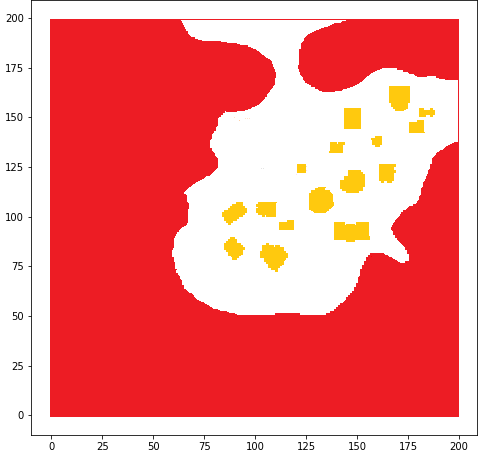
\includegraphics[width=.23\textwidth, height = 40mm]{obstacles.png}}
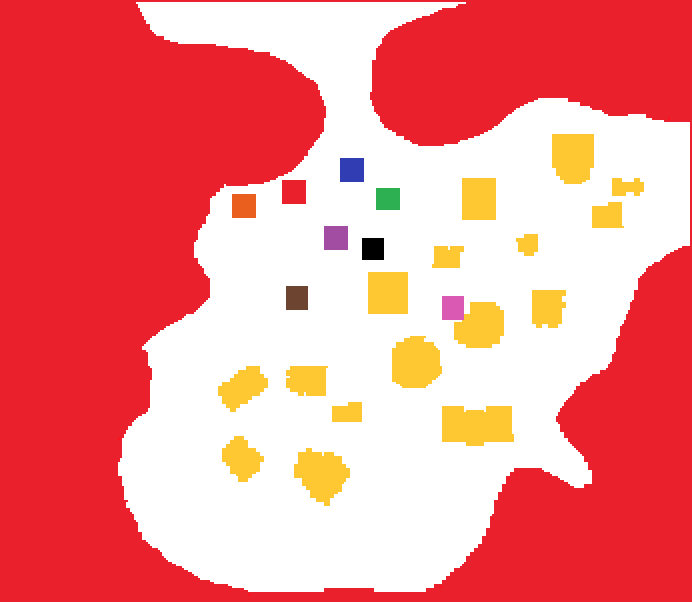
\includegraphics[width=.45\textwidth]{OnlineShield/start.png}
%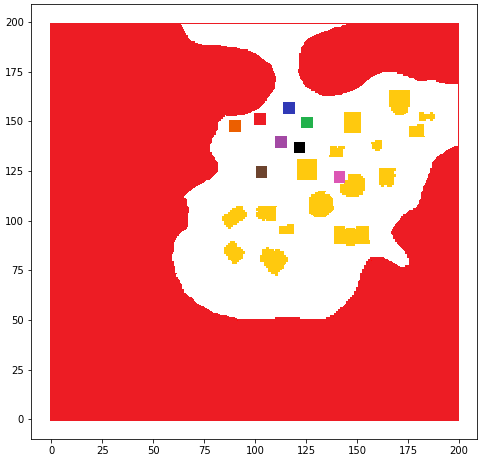
\includegraphics[]{grid.png}
}
\caption{(a) A custom Gazebo environment and (b) corresponding grid world representation where the yellow and red colored regions are unpassable terrain. The initial positions of the agents are marked by squares. }
\label{fig:sims}
\end{figure}

We tested two different scenarios in this environment. In the first scenario, we used a new safety function to prevent collision with obstacles (buildings) and ensure that the Manhattan distance between any two agents is at least 2 units. We randomly generated trajectories for the agents. We consider a scenario with eight agents in this environment. The even agents have the same trajectories, but in the opposite direction. The simulation with eight agents is presented in the video~\footnote{ The video can be found at https://tinyurl.com/yhdddpm6.}. For visual clarity, we present the original and the modified trajectories of six of the eight agents in Figure~\ref{fig:8agents}. The initial positions of the eight agents are marked in Figure~\ref{fig:sims}b.

In the second experiment, nine agents are occupying locations corresponding to a 3x3 square. The agent in the center has to escape the confinement. Further, no trajectories for the other agents are given. In this scenario, the central agent chooses its trajectory when it gets the highest priority. The agents along the path of this agent have to make way. During this process, sometimes a set of agents may actually have to make way for one another. This scenario can be seen in the video \footnote{The video can be found at https://tinyurl.com/ygwaplcp.}. We also provide the data for the trajectories and obstacles can be obtained \footnote{Numpy encodings of the trajectories and obstacles can be found at https://tinyurl.com/y6mkvcdx.}.


